\chapter{Koncepcja i~realizacja projektu}
\label{ch:koncepcja_i_realizacja}

\section{Założenia architektoniczne toru}
\label{sec:arch_zalozenia}

Architektura toru została zaprojektowana jako rozwiązanie strumieniowe, którego podstawowym zadaniem jest przetwarzanie danych TB przy zachowaniu stałej szerokości słowa 64-bit. Decyzje architektoniczne wynikają bezpośrednio z~przyjętych założeń projektowych (rozdz. \ref{ch:wymagania-i-narzedzia}) oraz z~charakterystyki kodowania LDPC, w~którym parametry kodowania mogą się zmieniać w~zależności od długości TB.

\subsection{Stała magistrala 64-bit jako oś projektu}
Cały tor oparto o~jednolity format przesyłania danych: słowa 64-bitowe w~kolejności MSB-first. Ujednolicenie szerokości interfejsu upraszcza integrację bloków i~umożliwia utrzymanie wysokiej przepustowości, jednak wprowadza istotne konsekwencje:
\begin{itemize}
    \item granice logiczne (koniec TB, granice CB, granice części systematycznej i~parzystości) mogą wypadać wewnątrz słowa 64-bit,
    \item konieczna jest jawna obsługa wyrównania i~dopełniania oraz przenoszenie informacji umożliwiającej odtworzenie dokładnej liczby bitów danych.
\end{itemize}
Z tego względu w~projekcie przewidziano mechanizmy pozwalające na jednoznaczną interpretację strumienia w~obecności \english{padding'u}.

\subsection{Uproszczony model sterowania strumieniem}
W celu ograniczenia złożoności pierwszej wersji projektu przyjęto jednokierunkowy handshake oparty o~sygnały \texttt{valid/last}, bez sygnału \texttt{ready}. Oznacza to, że blok odbierający dane ma obowiązek ich przyjęcia w~każdym cyklu z~\texttt{valid=1}. Taki model upraszcza połączenia pomiędzy etapami toru, ale jednocześnie wymusza odpowiednie podejście architektoniczne:
\begin{itemize}
    \item etapy przetwarzające dane „w locie” muszą być przeźroczyste w~sensie strumienia (brak możliwości zatrzymania źródła),
    \item etapy wymagające dostępu do większej ilości danych (np. operacje blokowe) muszą posiadać buforowanie, aby nie utracić danych wejściowych.
\end{itemize}
W projekcie dopuszczono zarówno strumień ciągły (1 słowo/cykl), jak i~wejście z~przerwami (\texttt{valid=0}), co zapewnia swobodę po stronie źródła danych.

\subsection{Przetwarzanie blokowe i~reset jako granica transakcji}
Aktualna wersja obsługuje pojedynczy TB pomiędzy resetami. Z punktu widzenia architektury reset pełni rolę granicy transakcji: po resecie układ przechodzi do stanu początkowego, zbiera dane TB, wykonuje pełne przetwarzanie, a~następnie kończy pracę na \texttt{out\_last}. Takie podejście upraszcza sterowanie i~zamykanie przetwarzania, a~także ułatwia weryfikację symulacyjną poprzez jednoznaczne odseparowanie przypadków testowych.

\subsection{Elastyczność kodowania LDPC}
Kodowanie LDPC w~5G NR może występować w~wielu konfiguracjach. W związku z~tym tor zaprojektowano jako konfigurowalny, tzn. zdolny do poprawnego przetwarzania TB dla różnych zestawów parametrów w~zakresie wspieranym przez implementację. Konsekwencją tej elastyczności jest konieczność:
\begin{itemize}
    \item przenoszenia metadanych konfiguracyjnych pomiędzy etapami toru,
    \item obsługi zmiennych długości bloków i~zmiennej liczby słów w~strumieniu wyjściowym,
    \item utrzymania spójnego formatu danych niezależnie od wybranej konfiguracji.
\end{itemize}

\subsection{Weryfikacja poprzez symulację i~syntezowalność}
Rozwiązanie opracowano tak, aby umożliwiało weryfikację bitowo-dokładną w~symulacji z~wykorzystaniem wektorów referencyjnych oraz aby było poprawnie syntezowalne dla zadanego układu FPGA. Raporty syntezy stanowią podstawę oceny wykorzystania zasobów i~parametrów czasowych, co pozwala formalnie ocenić wykonalność projektu w~warunkach narzuconych przez narzędzie syntezy.


\section{Struktura funkcjonalna i~przepływ danych}
\label{sec:struktura_i_przeplyw}

Przyjęta architektura stanowi tor przetwarzania danych, w~którym wejściowy TB jest przekształcany do postaci strumienia danych wyjściowych po operacjach przygotowania i~kodowania kanałowego. Tor ma charakter sekwencyjny: dane przechodzą przez kolejne etapy, a~każdy etap realizuje określoną funkcję w~procesie wytwarzania końcowego strumienia.

\subsection{Ogólny podział toru na etapy}
Z punktu widzenia funkcjonalnego tor można podzielić na następujące etapy:
\begin{enumerate}
    \item przyjęcie danych TB w~strumieniu 64-bit, wraz z~długością,
    \item obliczenie i~dołączenie sumy kontrolnej CRC,
    \item przygotowanie danych do kodowania LDPC:
    \begin{enumerate}
        \item obliczenie parametrów kodowania na podstawie długości TB,
        \item segmantacja TB na CB,
        \item obliczenie i~dołączenie sumy kontrolnej CRC do każdego CB.
    \end{enumerate}
    \item kodowanie LDPC i~wygenerowanie danych wyjściowych.
\end{enumerate}

\subsection{Przepływ danych wejściowych i~moment rozpoczęcia przetwarzania}
Dane wejściowe są dostarczane jako kolejne słowa 64-bitowe. Strumień może zawierać przerwy (cykle z~\texttt{in\_valid=0}), a~system rozpoznaje koniec TB na podstawie \texttt{in\_last=1} podanego wraz z~ostatnim ważnym słowem.

Ze względu na obecność etapów o~charakterze blokowym (w szczególności operacji zależnych od pełnej długości TB oraz parametrów kodowania), w~torze występuje faza zbierania danych, następnie przetwarzania, a~na końcu generowania danych wyjściowych. Dokładny moment rozpoczęcia emisji wyjścia zależy od długości TB, a~emisja danych wyjściowych nie może rozpocząć się przed odebraniem całej wiadomości na wejściu.

\subsection{Przepływ danych wewnątrz toru}
Między etapami przetwarzania dane są przekazywane jako strumień 64-bitowy z~semantyką \texttt{valid/last}. Wewnętrzne połączenia mogą dodatkowo przenosić metadane niezbędne do konfiguracji kodowania, w~szczególności takie, które zależą od długości TB i~wynikowego doboru parametrów LDPC.

Ważną cechą toru jest to, że część etapów musi operować na danych o~zmiennej długości (np. bloki o~długości zależnej od $Z_c$), podczas gdy interfejs transportuje dane w~stałych słowach 64-bit. Z tego względu na granicach etapów występują operacje składania/rozbijania danych bitowych oraz mechanizmy wyrównania.

\subsection{Strumień wyjściowy i~zakończenie przetwarzania}
Efektem działania toru jest strumień wyjściowy w~postaci słów 64-bitowych \texttt{out\_chunk}, oznaczonych \texttt{out\_valid}. Zakończenie przetwarzania całego TB jest sygnalizowane przez \texttt{out\_last=1} podane wraz z~ostatnim słowem wyjściowym.

Ze względu na stałą szerokość słowa, strumień wyjściowy może zawierać bity dopełnienia w~słowach brzegowych. Projekt udostępnia metadane umożliwiające jednoznaczną interpretację tych przypadków, sygnały \texttt{out\_pad\_left} oraz \texttt{out\_pad\_right} informują, które bity słowa są ważne.

\subsection{Warianty długości TB i~konsekwencje dla przepływu danych}
Architektura zakłada poprawną obsługę TB o~różnych długościach. Zmiana długości TB wpływa na:
\begin{itemize}
    \item liczbę słów wejściowych w~strumieniu,
    \item dobór parametrów kodowania LDPC,
    \item liczbę oraz rozmiar przetwarzanych bloków kodowych,
    \item liczbę słów w~strumieniu wyjściowym oraz wielkość \english{padding'u} w~słowach brzegowych.
\end{itemize}

W konsekwencji tor musi być przygotowany na to, że dla różnych przypadków testowych czas trwania przetwarzania oraz długość strumienia będą różne, mimo identycznego formatu interfejsu.


\section{Model strumieniowania i~buforowania danych}
\label{sec:strumieniowanie_buforowanie}

Tor przetwarzania oparto o~interfejs strumieniowy z~sygnałami \texttt{valid/last} bez sygnału \texttt{ready}. Oznacza to, że dane są przekazywane w~sposób jednokierunkowy: źródło sygnalizuje ważność słowa, a~odbiornik ma obowiązek je przyjąć. Taki model wpływa bezpośrednio na sposób organizacji modułów, konieczność buforowania oraz sposób obsługi przerw w~strumieniu wejściowym.

\subsection{Konsekwencje braku sygnału \texttt{ready}}
Brak \texttt{ready} oznacza, że blok odbiorczy nie może wymusić wstrzymania źródła danych. Z punktu widzenia architektury wymusza to spełnienie dwóch warunków:
\begin{itemize}
    \item każdy etap toru musi być w~stanie przyjąć dane zawsze, gdy poprzedni etap zgłasza \texttt{valid=1},
    \item jeżeli etap nie może przetworzyć danych w~locie, musi posiadać bufor umożliwiający ich zapis i~późniejsze przetwarzanie.
\end{itemize}

W praktyce oznacza to, że moduły w~torze dzielą się na:
\begin{itemize}
    \item \textbf{moduły przeźroczyste strumieniowo} -- przekazujące dane dalej w~tym samym cyklu (lub z~ustalonym, stałym opóźnieniem) przy zachowaniu semantyki \texttt{valid/last},
    \item \textbf{moduły blokowe} -- wymagające zebrania większej ilości danych i~dlatego wykorzystują buforowanie w~pamięci wewnętrznej.
\end{itemize}

\subsection{Buforowanie jako element architektury}
Zastosowanie buforów wynika z~charakterystyki przetwarzania: część operacji wymaga dostępu do danych w~sposób niedostępny w~czysto strumieniowym przetwarzaniu 1:1. Buforowanie w~projekcie pełni następujące role:
\begin{itemize}
    \item umożliwia zebranie danych wymaganych do wyznaczenia parametrów przetwarzania,
    \item umożliwia dostęp do wcześniej odebranych danych podczas formowania bloków o~zmiennej długości,
    \item umożliwia obliczenia wykonywane wielokrotnie na tych samych danych.
\end{itemize}

\subsection{Obsługa przerw w~strumieniu wejściowym}
Źródło danych może wprowadzać przerwy pomiędzy kolejnymi słowami TB, tj. występują cykle, w~których \texttt{in\_valid=0}. W takim przypadku:
\begin{itemize}
    \item układ nie próbuje próbkować \texttt{in\_chunk} ani nie zmienia stanu buforów danych,
    \item licznik odebranych słów/bitów jest zwiększany wyłącznie w~cyklach, w~których \texttt{in\_valid=1},
    \item koniec TB jest rozpoznawany dopiero w~cyklu, w~którym równocześnie \texttt{in\_valid=1} oraz \texttt{in\_last=1}.
\end{itemize}

Dzięki temu zachowanie toru nie zależy od tempa dostarczania danych, a~jedynie od ich kolejności oraz sygnałów sterujących.

\subsection{Deterministyczność przepływu}
Model \texttt{valid/last} bez \texttt{ready} oraz jawne buforowanie powodują, że przepływ danych jest deterministyczny: kolejność słów w~buforach oraz kolejność emisji na wyjściu zależą wyłącznie od kolejności nadejścia danych oraz metadanych. W połączeniu z~weryfikacją symulacyjną umożliwia to jednoznaczne porównywanie strumienia wyjściowego z~wektorami referencyjnymi.


\section{Cykliczny kod nadmiarowy (CRC)}
\label{sec:CRC}

W torze nadawczym 5G NR suma kontrolna CRC jest dopisywana do TB przed dalszymi etapami przetwarzania. W projekcie zastosowano dwustopniowe podejście do realizacji CRC:
\begin{itemize}
    \item najpierw opracowano moduł szeregowy działający bit-po-bicie (\texttt{crc\_serial}),
    \item następnie rozbudowano rozwiązanie do postaci równoległej 64-bit (\texttt{crc\_tb\_parallel}), wykorzystując kombinacyjną aktualizację CRC o~całe słowo (\texttt{crc\_update}) oraz ponownie używając \texttt{crc\_serial} do obsługi niepełnej końcówki TB.
\end{itemize}

Schemat blokowy rozwiązania przedstawiono na rys. \ref{fig:crc_serial_overview} oraz \ref{fig:crc_tb_overview}.

\begin{figure}[!ht]
\centering
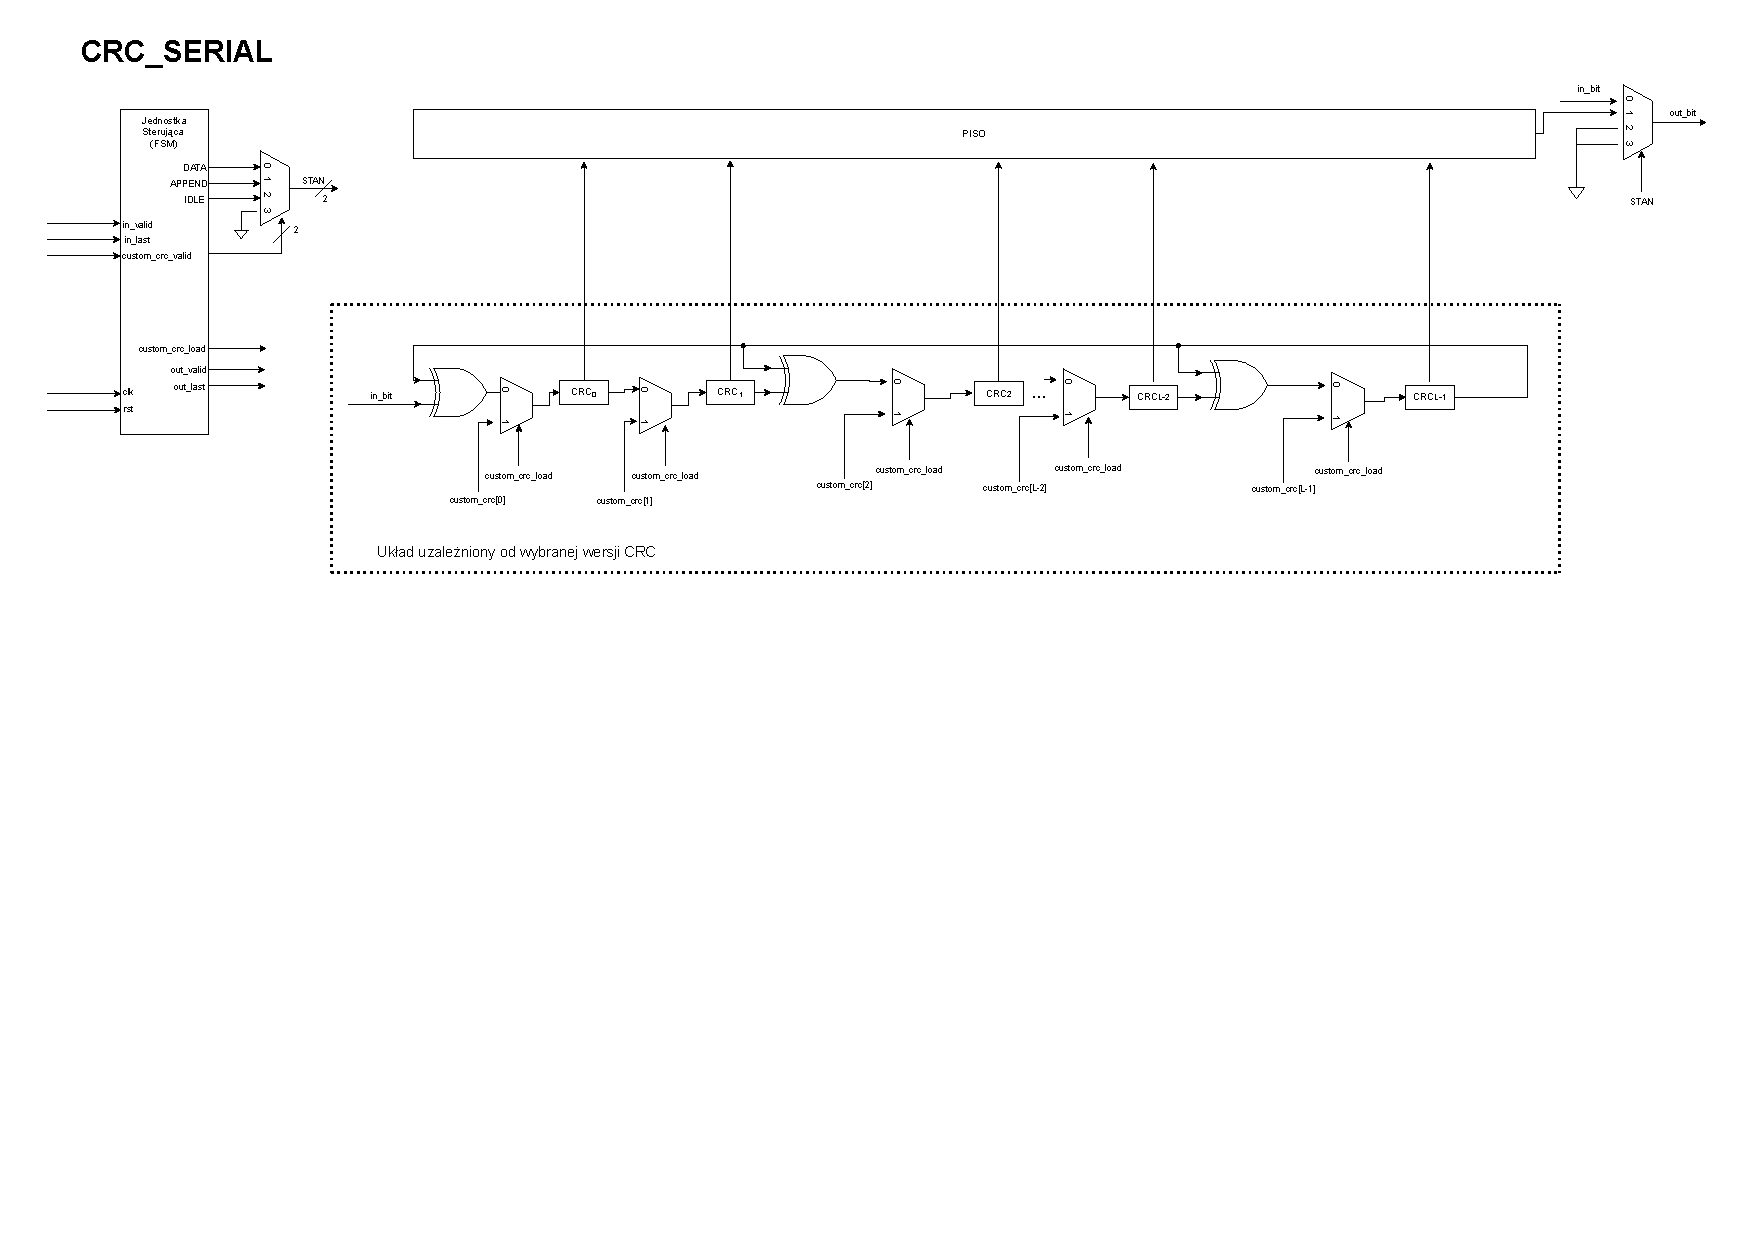
\includegraphics[width=0.98\linewidth]{./schematy/CRC_SERIAL.pdf}
\caption{Schemat blokowy modułu \texttt{crc\_serial} liczącego CRC szeregowo.}
\label{fig:crc_serial_overview}
\end{figure}

\begin{figure}[!ht]
\centering
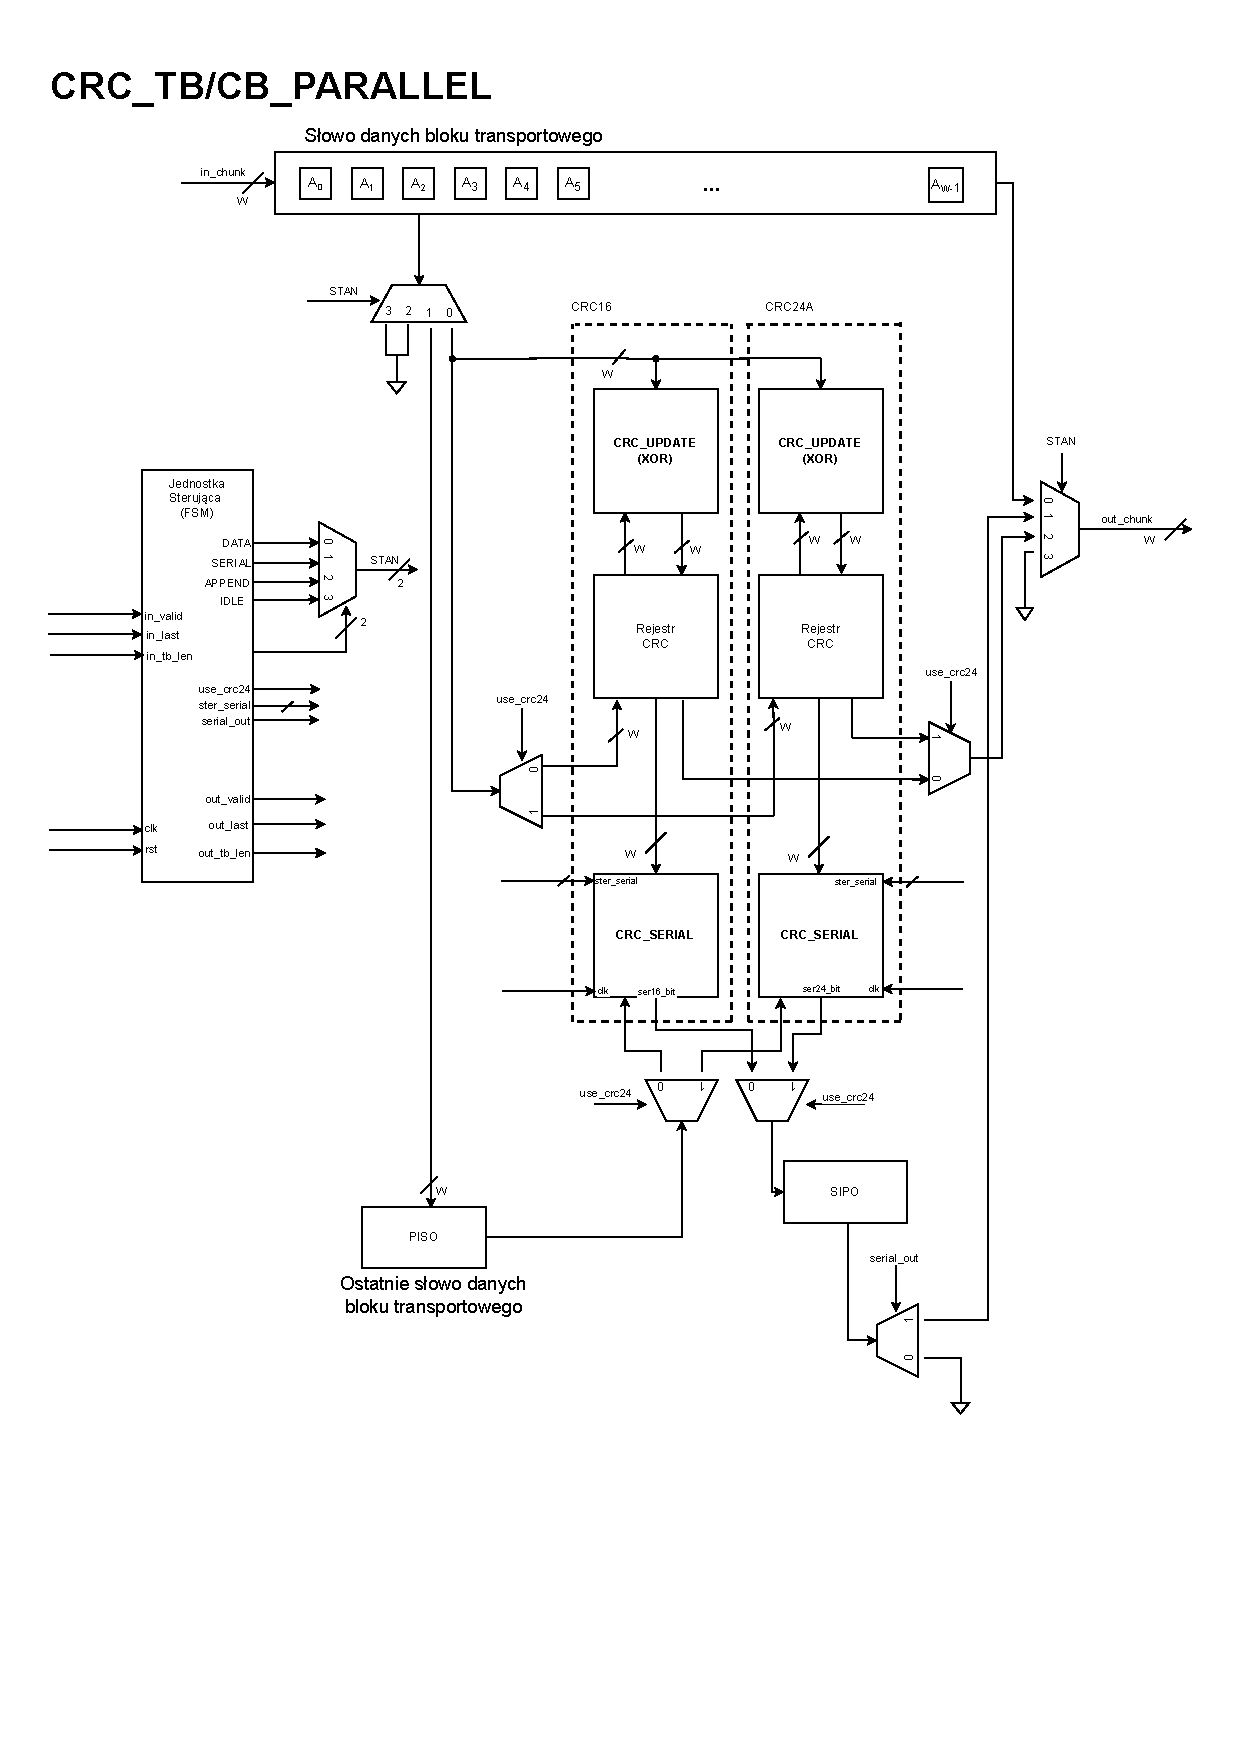
\includegraphics[width=0.98\linewidth]{./schematy/CRC_TB.pdf}
\caption{Schemat blokowy modułu \texttt{crc\_tb\_parallel} liczącego CRC równolegle.}
\label{fig:crc_tb_overview}
\end{figure}



% -----------------------------------------------------------------------------

\subsection{Wariant bazowy: moduł szeregowy \texttt{crc\_serial}}
\label{subsec:crc_serial}

Moduł \texttt{crc\_serial} realizuje obliczanie CRC w~sposób klasyczny, tj. aktualizuje rejestr CRC o~jeden bit na cykl zegara i~jednocześnie przepuszcza strumień danych na wyjście. Po zakończeniu danych wejściowych moduł dopisuje na wyjściu kolejne bity CRC, a~sygnał \texttt{out\_last} występuje tylko raz -- na ostatnim bicie CRC. Interfejs modułu jest bitowy (1 bit/cykl) i~wykorzystuje sterowanie \texttt{valid/last}.

Wewnątrz \texttt{crc\_serial} zastosowano rejestr CRC o~długości zależnej od parametru \texttt{L}. W aktualnej wersji przewidziano wszystkie warianty używane w~standardzie 5G NR:
\begin{itemize}
    \item CRC16 -- używany dla TB o~długości mniejszej lub równej 3824 bitów,
    \item CRC24A -- używany dla TB o~długości większej niż 3824 bity,
    \item CRC24B -- używany dla CB.
\end{itemize}

Kod źródłowy modułu znajduję się w~pliku \texttt{crc\_serial.v}.

\subsection{Rozszerzenie modułu szeregowego o~inicjalizację stanu CRC}
\label{subsec:crc_serial_custom_init}

W praktycznej integracji CRC w~torze równoległym pojawia się potrzeba podania stanu początkowego rejestru CRC, który odpowiada obliczeniom wykonanym wcześniej na pełnych słowach 64-bitowych. Z tego powodu moduł \texttt{crc\_serial} został rozszerzony o~wejścia:
\begin{itemize}
    \item \texttt{custom\_crc} --- wartość stanu CRC, od której ma rozpocząć się dalsze liczenie,
    \item \texttt{custom\_crc\_valid} --- sygnał wyboru (gdy aktywny, stan startowy nie jest zerowany, tylko ładowany z~\texttt{custom\_crc}).
\end{itemize}

Rozszerzenie to umożliwia użycie \texttt{crc\_serial} jako kontynuacji obliczeń w~sytuacji, gdy część TB została już przetworzona równolegle, a~pozostała jedynie niepełna końcówka wymagająca operacji bitowych.

% -----------------------------------------------------------------------------

\subsection{Moduł \texttt{crc\_update}: równoległa aktualizacja CRC o~64 bity}
\label{subsec:crc_update}

Aby umożliwić pracę w~torze 64-bitowym bez iteracji bit-po-bicie dla każdego słowa, zastosowano moduł \texttt{crc\_update}. Jest to blok kombinacyjny, który wyznacza:
\[
CRC_{next} = f(CRC_{in},\; data[63:0])
\]
gdzie funkcja $f(\cdot)$ jest zależnością liniową w~ciele $GF(2)$ (realizowaną jako XOR wybranych bitów stanu i~danych).

Podejście to odpowiada koncepcji generatorów CRC równoległych, w~których stan następny jest funkcją aktualnego stanu oraz równoległego wektora danych \cite{bib:stavinov2010_parallel_crc_gen}.

Kod źródłowy modułu znajduję się w~pliku \texttt{crc\_update.v}.


\subsection{Generowanie równań XOR na podstawie macierzy H1 i~H2}
\label{subsec:crc_update_generation}

Równoległą aktualizację CRC można wyznaczyć z~własności liniowości obliczeń w~$GF(2)$. Najpierw buduje się dwie macierze zależności:
\begin{itemize}
  \item $H1$ opisuje, jak każdy bit wejściowego słowa danych wpływa na poszczególne bity CRC na wyjściu przy zerowym stanie początkowym CRC,
  \item $H2$ opisuje, jak każdy bit początkowego stanu CRC wpływa na poszczególne bity CRC na wyjściu przy słowie danych składającym się z~samych zer.
\end{itemize}

Następnie dla każdego bitu CRC na wyjściu odczytuje się z~tych macierzy, które wejścia mają na niego wpływ. W praktyce wygląda to tak, że:
\begin{itemize}
  \item jedynki w~odpowiedniej kolumnie $H1$ wskazują, które bity danych należy zsumować operacją XOR,
  \item jedynki w~odpowiedniej kolumnie $H2$ wskazują, które bity bieżącego stanu CRC należy również dołączyć do XOR.
\end{itemize}

Ostatecznie każdy bit jest XOR-em wybranych bitów danych oraz wybranych bitów stanu CRC. Zestaw takich równań stanowi gotową postać kombinacyjną aktualizacji CRC o~całe słowo danych w~jednym kroku.



W projekcie zastosowano skrypt MATLAB:
\begin{itemize}
    \item \texttt{gen\_parallel\_crc\_matrix.m} --- wyznacza macierze $H1/H2$ dla zadanych wielomianów (CRC16, CRC24A, CRC24B) i~generuje linie równań XOR w~postaci nadającej się do przeniesienia do kodu HDL.
\end{itemize}

W efekcie moduł \texttt{crc\_update} zawiera funkcje (dla odpowiednich wariantów CRC), w~których każda linia ma postać:
\[
crc\_out[i] = \bigoplus(\text{wybrane bity } crc\_in \text{ oraz } data)
\]
co odpowiada dokładnie 64 krokom aktualizacji szeregowej wykonanym w~jednym cyklu.

% -----------------------------------------------------------------------------

\subsection{Moduł \texttt{crc\_tb\_parallel}: integracja trybu równoległego i~szeregowego}
\label{subsec:crc_tb_parallel}

Moduł \texttt{crc\_tb\_parallel} stanowi właściwą implementację CRC w~torze 64-bitowym. Dla kolejnych słów wejściowych:
\begin{itemize}
    \item przekazuje dane na wyjście 1:1,
    \item równolegle aktualizuje rejestr CRC o~64 bity na podstawie \texttt{crc\_update}.
\end{itemize}

Po wykryciu końca TB (\texttt{in\_last=1}) moduł przechodzi do dopisania CRC. W zależności od tego, czy ostatnie słowo TB jest pełne, stosowane są dwa tryby pracy (zgodne z~ideą pokazaną na rys. \ref{fig:crc_tb_overview}).

Kod źródłowy modułu znajduję się w~pliku \texttt{crc\_tb\_parallel.v}. Kod źródłowy modułu liczącego CRC dla CB znajduje się w~pliku \texttt{crc\_cb\_parallel.v} (działa na tej samej zasadzie, ale obsługuje tylko CRC24B).

\subsection{Dobór długości CRC na podstawie długości TB}
\label{subsec:crc_len_select}

Wybór wariantu CRC jest realizowany na podstawie długości TB:
\begin{itemize}
    \item dla \texttt{in\_tb\_len > 3824} wybierany jest wariant CRC24A,
    \item dla \texttt{in\_tb\_len <= 3824} wybierany jest wariant CRC16.
\end{itemize}

\subsection{Wyznaczenie końcówki TB (``ogona'') na podstawie \texttt{tb\_len}}
\label{subsec:tail_calc}

Istotnym założeniem projektu jest to, że na wejściu nie jest podawana informacja o~dopełnieniu ostatniego słowa (padding). Zamiast tego moduł wykorzystuje \texttt{tb\_len}, aby wyznaczyć liczbę ważnych bitów w~ostatnim słowie TB:
\begin{itemize}
    \item obliczane jest \texttt{rem = tb\_len mod 64},
    \item jeżeli \texttt{rem=0}, ostatnie słowo ma 64 ważne bity,
    \item w~przeciwnym razie ostatnie słowo ma \texttt{rem} ważnych bitów.
\end{itemize}

Dzięki temu wystarczające jest przekazanie samej długości TB w~bitach, a~źródło danych nie musi raportować osobno ile bitów w~ostatnim słowie jest ważnych. Z tej samej przyczyny na wyjściu modułu CRC nie jest przekazywana informacja o~paddingu ostatniego słowa -- długość TB pozostaje znana i~niezmienna (moduł przekazuje \texttt{out\_tb\_len} bez CRC jako metadane ramki).

\subsection{Tryb S\_APPEND: ostatnie słowo pełne}
\label{subsec:append_mode}

Jeżeli ostatnie słowo TB jest pełne (64 ważne bity), to po jego wypuszczeniu moduł:
\begin{itemize}
    \item emituje osobne słowo 64-bit zawierające CRC umieszczone w~najbardziej znaczących bitach,
    \item pozostałe bity słowa CRC są zerowane,
    \item \texttt{out\_last} jest ustawiane przy tym słowie CRC (kończąc całą ramkę).
\end{itemize}

Takie rozwiązanie upraszcza dopisanie CRC, ponieważ nie jest wymagane mieszanie końcówki danych z~CRC w~jednym słowie.

\subsection{Tryb S\_SERIAL: ostatnie słowo niepełne}
\label{subsec:serial_mode}

Jeżeli ostatnie słowo TB jest niepełne, konieczne jest potraktowanie pozostałych bitów końcówki jako strumienia bitowego i~dopisanie CRC w~sposób zapewniający poprawną kolejność bitów oraz wyrównanie do granicy 64 bitów.

W tym celu \texttt{crc\_tb\_parallel}:
\begin{itemize}
    \item przełącza się na ścieżkę bitową,
    \item uruchamia \texttt{crc\_serial} jako moduł pomocniczy,
    \item ładuje do \texttt{crc\_serial} stan CRC wyliczony wcześniej na pełnych słowach 64-bit (sygnały \texttt{custom\_crc/custom\_crc\_valid}),
    \item podaje do \texttt{crc\_serial} kolejne bity ostatniego słowa (MSB-first) i~oznacza ostatni bit danych zgodnie z~wyliczoną liczbą ważnych bitów,
    \item odbiera strumień bitowy zawierający końcówkę danych + CRC i~składa go z~powrotem do słów 64-bit.
\end{itemize}

Jeżeli suma liczby bitów (końcówka danych + CRC) przekracza 64, wyjście tworzy dwa słowa 64-bit (wyrównanie do 128 bitów). W przeciwnym wypadku powstaje jedno słowo wyjściowe, dopełnione zerami do pełnych 64 bitów.

% -----------------------------------------------------------------------------

\subsection{Podsumowanie roli CRC w~torze}
\label{subsec:crc_summary}

Zastosowana architektura CRC łączy prostotę implementacji szeregowej z~wydajnością przetwarzania równoległego:
\begin{itemize}
    \item pełne słowa 64-bitowe przetwarzane są w~jednym cyklu przez \texttt{crc\_update},
    \item wyłącznie niepełna końcówka TB wymaga pracy bitowej, zrealizowanej przez ponowne użycie \texttt{crc\_serial},
    \item \texttt{tb\_len} eliminuje potrzebę przekazywania informacji o~paddingu na wejściu.
\end{itemize}

To podejście pozwala zachować spójny format danych w~całym torze przy jednoczesnym zachowaniu bitowo-dokładnej zgodności z~referencją.


\section{Przygotowanie danych do kodowania LDPC}
\label{sec:ldpc_prep}

Etap przygotowania danych do kodowania LDPC realizuje moduł \texttt{LDPC\_prep}. Jego zadaniem jest przekształcenie wejściowego strumienia TB do postaci sekwencji CB gotowych do podania na wejście kodera LDPC wraz z~kompletem metadanych konfiguracyjnych (BG, $Z_c$, $k$, liczba \english{filler bits}). Moduł odpowiada za wyznaczenie parametrów wynikających ze standardowych reguł, segmentację TB na CB, obliczenie i~dopisanie CRC (jeśli wymagane), oraz przygotowanie strumienia wyjściowego przy zachowaniu stałej szerokości 64 bitów.

Schemat blokowy rozwiązania przedstawiono na rys. \ref{fig:ldpc_prep_overview}, a~kod źródłowy znajduję się w~pliku \texttt{LDPC\_prep.v}.

\begin{figure}[!ht]
\centering
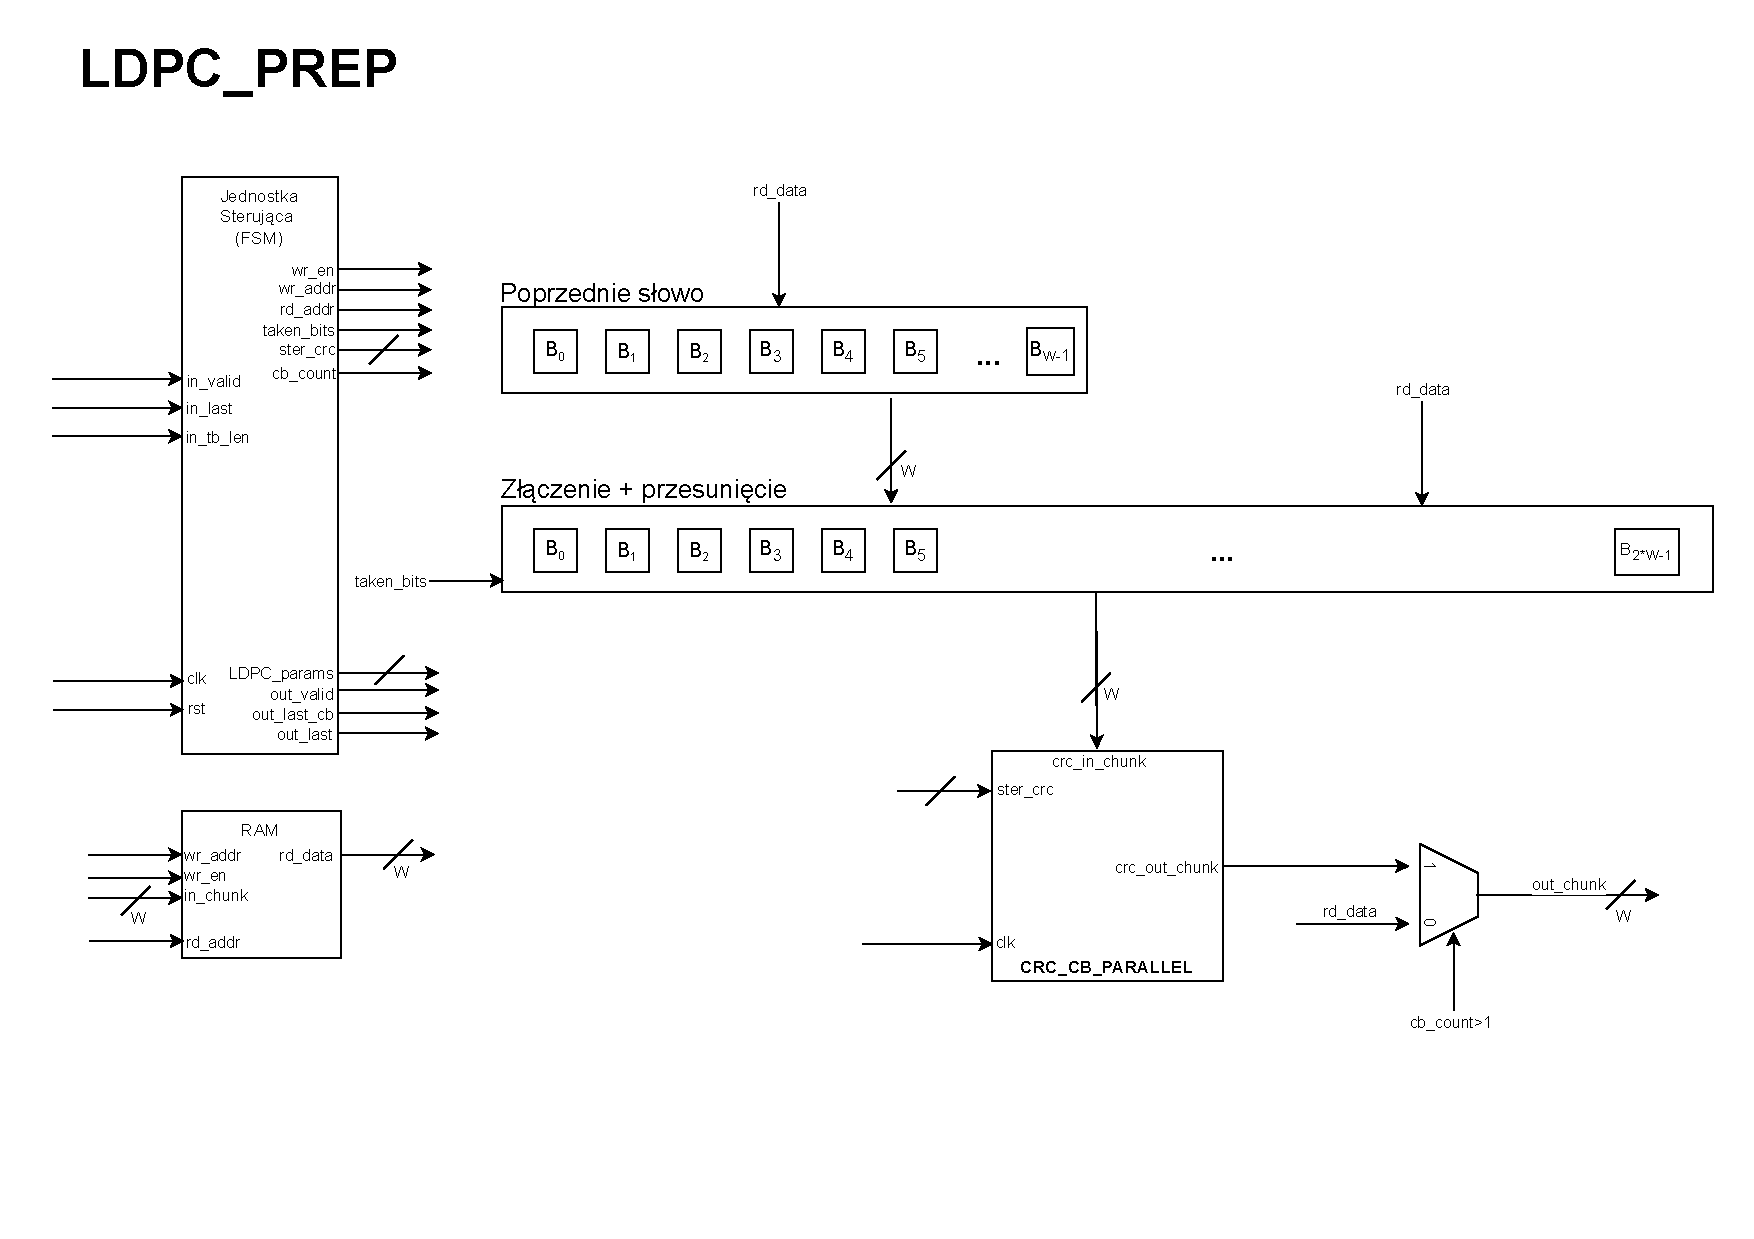
\includegraphics[width=0.98\linewidth]{./schematy/LDPC_PREP.pdf}
\caption{Schemat blokowy modułu \texttt{LDPC\_prep} przygotowującego dane do kodowania LDPC.}
\label{fig:ldpc_prep_overview}
\end{figure}

.


\subsection{Buforowanie TB i~rozdzielenie faz pracy}
\label{subsec:ldpc_prep_buffering}

Ponieważ przygotowanie CB wymaga operowania na danych o~zmiennej długości oraz wyznaczenia parametrów zależnych od całej ramki, moduł \texttt{LDPC\_prep} w~pierwszym kroku buforuje cały TB w~pamięci wewnętrznej słowami 64-bit. Dane są zapisywane wyłącznie w~cyklach, w~których \texttt{in\_valid=1}, a~koniec TB jest wykrywany poprzez \texttt{in\_last=1} podane razem z~ostatnim ważnym słowem. Przerwy w~strumieniu wejściowym (\texttt{in\_valid=0}) nie wpływają na poprawność działania --- powodują jedynie wydłużenie fazy odbioru.

W konsekwencji praca modułu jest naturalnie podzielona na trzy fazy:
\begin{itemize}
  \item \textbf{faza odbioru} -- zapis TB do pamięci RAM,
  \item \textbf{faza przygotowania} -- obliczenie parametrów segmentacji i~LDPC,
  \item \textbf{faza segmentacji i~emisji} -- odczytanie odpowiednich fragmentów TB, dopisanie CRC (jeśli wymagane) oraz emisja bloków kodowych jako strumień 64-bit.
\end{itemize}

\subsection{Wyznaczenie parametrów CRC i~wielkości pośrednich}
\label{subsec:ldpc_prep_crc_b}

Na podstawie długości \texttt{tb\_len} wyznaczana jest długość CRC dla TB (16 lub 24 bity) oraz wielkość pośrednia:
\[
B = \mathrm{TB} + \mathrm{CRC}_{TB}
\]
czyli liczba bitów po dopisaniu CRC dla TB. Informacja \texttt{tb\_len} jest wystarczająca do dalszych obliczeń i~do wyznaczania końcówek (bitów niepełnych słów) --- nie jest wymagane przekazywanie oddzielnej informacji o~\english{padding'u} ostatniego słowa na wejściu.

\subsection{Segmentacja TB na CB}
\label{subsec:ldpc_prep_segmentation}

Jeżeli długość $B$ przekracza dopuszczalny rozmiar pojedynczego CB dla wybranego grafu bazowego, moduł wyznacza liczbę bloków kodowych $C$ oraz długości pośrednie używane do przygotowania CB. W przypadku segmentacji uwzględniany jest narzut CRC dla CB (CRC24B), co powoduje powstanie wielkości:
\[
B' = B + C \cdot \mathrm{CRC}_{CB}
\]

Następnie wyznaczana jest ilość danych przypadającej na jeden CB. Wartość $k_{CB}$ zależy od tego, czy występuje segmentacja:
\[
k_{CB} =
\begin{cases}
B, & C = 1 \\
\left\lceil \dfrac{B'}{C} \right\rceil, & C > 1
\end{cases}
\]
gdzie $B$ oznacza długość bloku po dopisaniu CRC dla TB, natomiast $B' = B + C \cdot \mathrm{CRC}_{CB}$ uwzględnia dodatkowy narzut CRC24B dopisywany do każdego CB w~przypadku segmentacji.


W projekcie obliczenia wymagające dzielenia z~zaokrągleniem w~górę (np. dla $C$ oraz długości danych CB) realizowane są sprzętowo przez pomocniczy moduł \texttt{Ceil}. Realizuje on dzielenie w~sposób iteracyjny, metodą kolejnych odejmowań. Po uruchomieniu  wartości licznika i~mianownika zatrzaskiwane są do rejestrów roboczych, a~następnie w~każdym cyklu odejmuje mianownik od bieżącej wartości licznika i~jednocześnie inkrementuje licznik ilorazu. Iteracje trwają aż do momentu, gdy pozostała wartość jest mniejsza od mianownika -- wtedy moduł przechodzi do stanu wyniku, zapamiętuje resztę i~wystawia iloraz jako liczbę wykonanych odejmowań. Sygnał \texttt{result\_valid} informuje o~gotowości wyniku; wynik jest podawany tak długo, jak utrzymywane jest \texttt{enable=1}, a~zwolnienie \texttt{enable} powoduje powrót do stanu bezczynności i~gotowość do kolejnego obliczenia. Z uwagi na iteracyjny charakter (jedno odejmowanie na cykl) moduł ma zmienną latencję zależną od wartości ilorazu. Latencja (opóźnienie przetwarzania) oznacza czas (liczbę cykli zegara) pomiędzy dostarczeniem danych na wejście układu, a~pojawieniem się odpowiadających im danych na wyjściu.


\textbf{Uwaga projektowa:} w~aktualnej wersji dobór grafu bazowego jest podyktowany wyłącznie długością bloku transportowego. Jest to świadome uproszczenie interfejsu, ponieważ do pełnego doboru BG w~5G NR potrzebne są dodatkowe parametry, które nie są dostarczane na wejściu modułu, ponieważ nie są one częścią tej implementacji. W praktyce dobór BG może być realizowany przez nadrzędny system sterujący, który zna pełen kontekst transmisji.

\subsection{Dobór $Z_c$, wyznaczenie $k$ oraz liczby $filler$ $bits$}
\label{subsec:ldpc_prep_zc_k_filler}

Po wyznaczeniu długości danych przypadającej na pojedynczy CB moduł określa parametry wymagane do skonfigurowania kodera LDPC. W tym miejscu istotne jest rozróżnienie dwóch pojęć, które bywają opisywane podobnymi symbolami, natomiast w~implementacji pełnią różne role:

\begin{itemize}
  \item \textbf{$k_b$ (zmienne)} -- liczba „bloków danych” potrzebnych do przeniesienia aktualnej długości informacji w~CB; wartość ta zależy od wybranego grafu bazowego oraz od długości danych. Jest ona wykorzystywana do wyznaczenia minimalnej wymaganej wartości $Z_c$.
  \item \textbf{$K_b$ (stałe dla grafu)} -- docelowa liczba bloków danych wynikająca bezpośrednio z~grafu bazowego. Dla BG1 jest ona stała i~wynosi $K_b=22$, natomiast dla BG2 wynosi $K_b=10$.
\end{itemize}

Najpierw wyznaczana jest minimalna wartość $Z_c$ zapewniająca możliwość umieszczenia danych w~CB przy zadanym $k_b$:
\[
Z_{c,\min} = \left\lceil \frac{k_{CB}}{k_b} \right\rceil
\]
a następnie dobierane jest docelowe $Z_c$ z~listy dopuszczalnych wartości (co zapewnia zgodność ze zdefiniowanymi w~standardzie rozmiarami podmacierzy).

Po ustaleniu $Z_c$ wyznaczana jest docelowa długość części systematycznej kodu, wynikająca ze struktury grafu bazowego:
\[
k = Z_c \cdot K_b
\]
gdzie $K_b$ jest stałe dla danego BG. Oznacza to, że w~przypadku BG2 nawet wtedy, gdy z~obliczeń wynika $k_b < 10$, długość $k$ pozostaje równa $Z_c \cdot 10$, a~„brakujące” bloki danych są wypełniane bitami typu \english{filler}.

Liczba bitów dopełniających jest wyznaczana jako:
\[
N_\mathrm{filler} = k - k_{CB}
\]
i w~module jest udostępniana na wyjściu jako \texttt{out\_filler\_cnt}. Wartość ta określa, ile bitów w~części systematycznej CB nie niesie informacji użytkownika i~powinno zostać wypełnionych zgodnie z~przyjętą w~torze konwencją.


\subsection{Formowanie strumienia wyjściowego CB na szynie 64-bit}
\label{subsec:ldpc_prep_streaming}

Wyjście \texttt{LDPC\_prep} stanowi strumień słów 64-bit zawierających dane kolejnych bloków kodowych. Moduł zapewnia poprawne przejścia granic bitowych CB nawet wtedy, gdy granice CB wypadają wewnątrz słowa 64-bit w~buforze TB. W tym celu wykorzystywane jest składanie słów na podstawie pary kolejnych słów bufora oraz przesunięcia bitowego, tak aby uzyskać ciągły strumień bitów CB w~konwencji MSB-first.

W zależności od liczby bloków kodowych występują dwa przypadki:
\begin{itemize}
  \item \textbf{Pojedynczy CB ($C=1$):} moduł emituje zawartość bufora TB słowo-po-słowie. W tym wariancie nie występuje CRC dla CB (zgodnie z~regułą, że CRC24B jest stosowane dopiero przy segmentacji).
  \item \textbf{Wiele CB ($C>1$):} dla każdego CB moduł pobiera z~bufora odpowiednią liczbę bitów danych, a~następnie dopisuje CRC24B dla CB i~emituje wynik jako strumień 64-bit.
\end{itemize}

Granice bloków CB na wyjściu są sygnalizowane przez:
\begin{itemize}
  \item \texttt{out\_last\_chunk} --- znacznik ostatniego słowa bieżącego CB,
  \item \texttt{out\_last\_cb} --- znacznik ostatniego CB w~całym TB.
\end{itemize}

\subsection{Dopisanie CRC24B dla CB}
\label{subsec:ldpc_prep_crc_cb}

Dla przypadku segmentacji ($C>1$) moduł dopisuje CRC dla każdego bloku kodowego (CRC24B) przy użyciu bloku \texttt{crc\_cb\_parallel}. Funkcjonalnie moduł ten jest odpowiednikiem \texttt{crc\_tb\_parallel} (opisanym w~sekcji \ref{sec:CRC}) --- pracuje na szynie 64-bit i~realizuje dopisanie CRC do strumienia danych, z~obsługą sytuacji, gdy końcówka danych CB nie kończy się na granicy słowa 64-bit. Z tego względu w~niniejszym rozdziale nie powiela się pełnego opisu wewnętrznej struktury CRC dla CB; można odwołać się do schematu i~mechanizmów przedstawionych w~sekcji \ref{sec:CRC}.

\subsection{Metadane konfiguracyjne przekazywane do kodera LDPC}
\label{subsec:ldpc_prep_metadata}

Wraz z~danymi CB moduł generuje metadane wymagane do skonfigurowania kodera LDPC:
\begin{itemize}
  \item \texttt{out\_k} --- docelowa długość bloku kodowego po dopełnieniu,
  \item \texttt{out\_zc} --- dobrana wartość $Z_c$,
  \item \texttt{out\_bg} --- wybrany graf bazowy (1 oznacza graf bazowy 1, 0 oznacza graf bazowy 2),
  \item \texttt{out\_filler\_cnt} --- liczba bitów dopełniających.
\end{itemize}

\section{Implementacja kodera LDPC}
\label{sec:ldpc_encoder_impl}

Najważniejszym blokiem toru jest moduł \texttt{LDPC\_encode}, realizujący kodowanie QC-LDPC na poziomie pojedynczych bloków kodowych w~stałym formacie strumieniowym 64-bit. Moduł został zaprojektowany jako rozwiązanie elastyczne: dla zadanych parametrów (\texttt{BG}, $Z_c$, $k$, $filler$ $bits$) potrafi zakodować CB zgodnie z~regułami grafów bazowych 5G NR oraz wygenerować strumień bitów kodowych, zachowując 64-bitową magistralę danych na wejściu i~wyjściu.

Schemat blokowy kodera przedstawiono na rys. \ref{fig:ldpc_encode_overview}, a~kod źródłowy znajduje się w~pliku \texttt{LDPC\_encode.v}.

\begin{figure}[!ht]
\centering
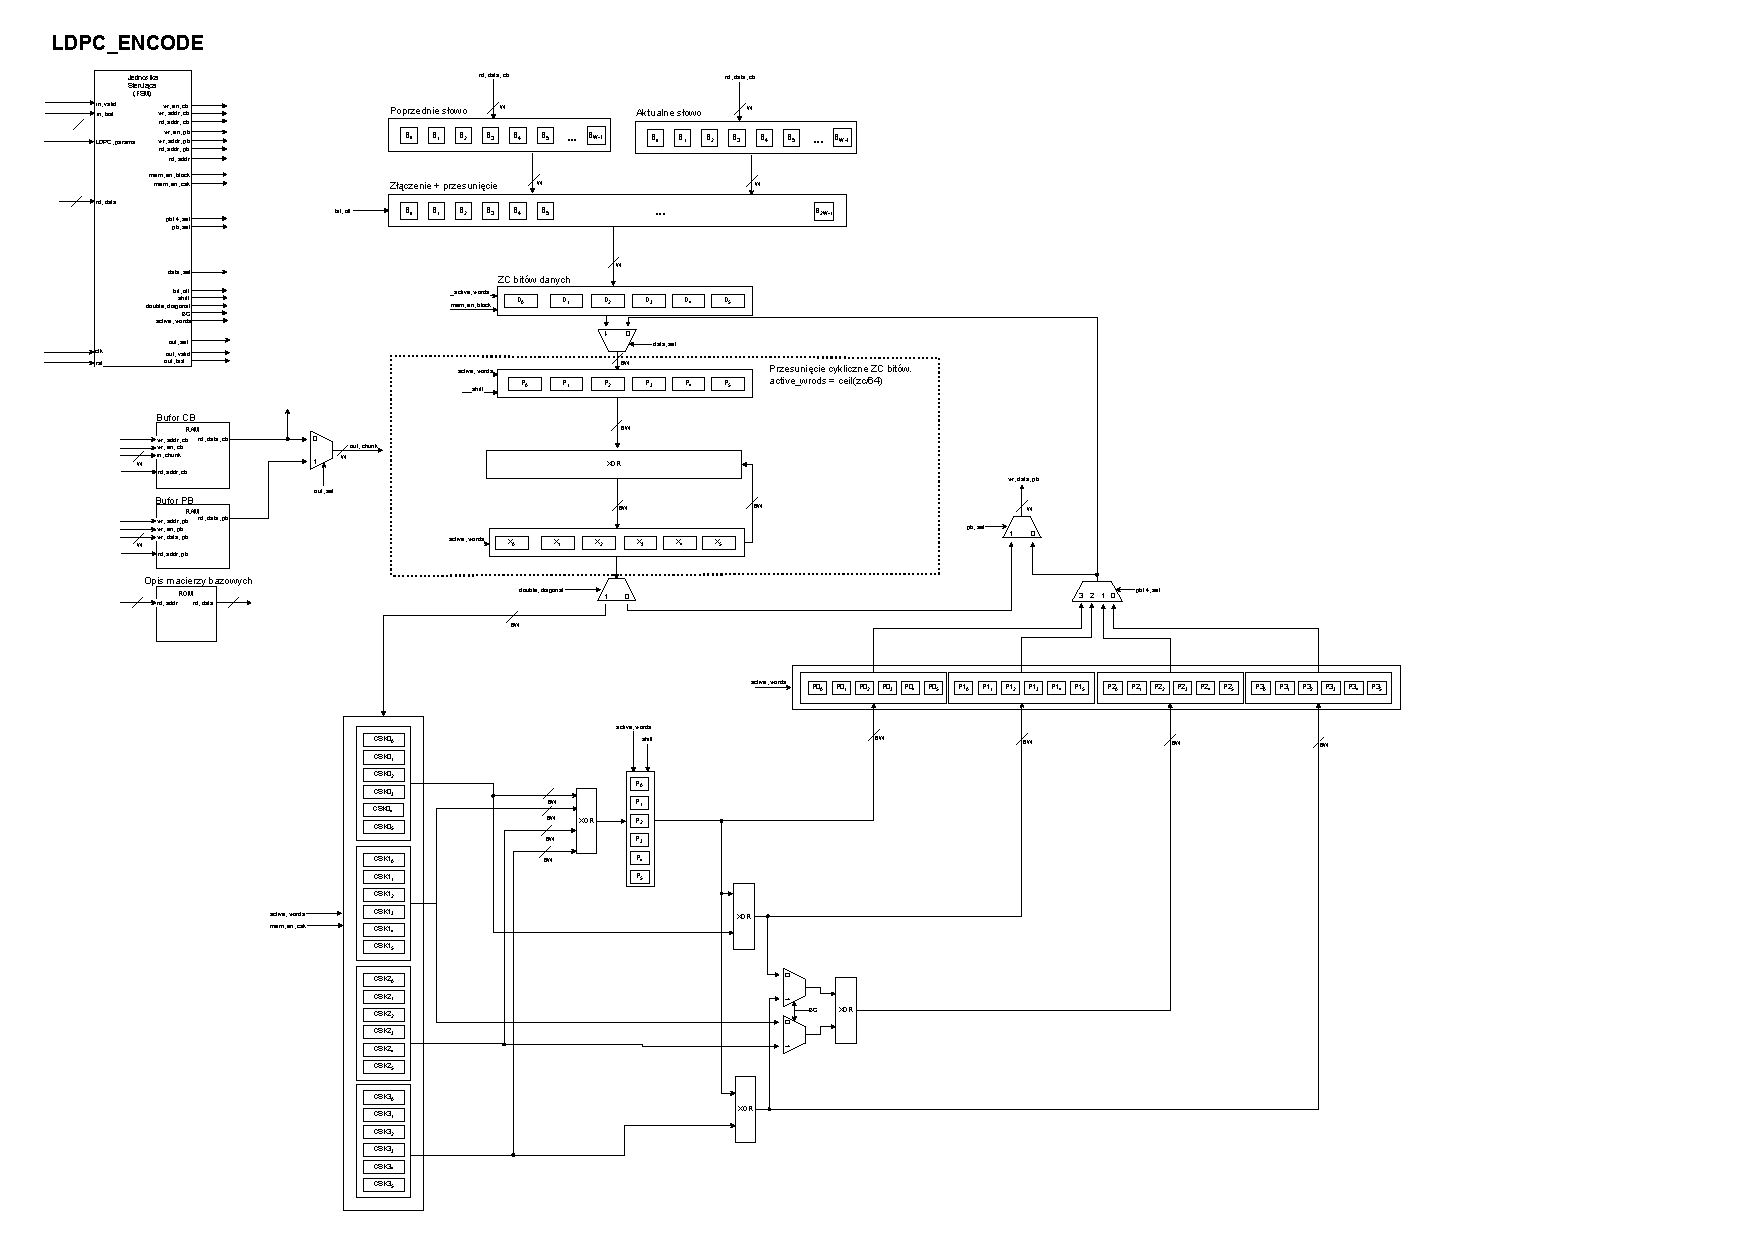
\includegraphics[width=0.98\linewidth]{./schematy/LDPC_ENCODE.pdf}
\caption{Schemat blokowy modułu \texttt{LDPC\_encode}.}
\label{fig:ldpc_encode_overview}
\end{figure}

% -----------------------------------------------------------------------------

\subsection{Interfejs wejściowy i~buforowanie danych}
\label{subsec:ldpc_enc_input_buffering}

Wejście kodera stanowi strumień słów 64-bit sterowany sygnałami \texttt{in\_valid/in\_last} oraz metadanymi konfiguracyjnymi:
\begin{itemize}
    \item \texttt{in\_k} -- docelowa długość części systematycznej $k$ dla CB,
    \item \texttt{in\_zc} -- rozmiar podmacierzy,
    \item \texttt{in\_bg} -- wybór grafu bazowego (BG1/BG2),
    \item \texttt{in\_filler\_cnt} -- liczba \english{filler bits} w~CB.
\end{itemize}

Z uwagi na brak sygnału \texttt{ready}, przyjęto model, w~którym dane są próbkowane zawsze, gdy \texttt{in\_valid=1}, a~źródło ma obowiązek podać stabilne \texttt{in\_chunk} w~cyklu ważności. Moduł dopuszcza przerwy w~strumieniu (\texttt{in\_valid=0}) -- skutkują one jedynie wydłużeniem czasu buforowania.

W pierwszej fazie pracy koder buforuje cały CB w~pamięci wewnętrznej słowami 64-bit. Granice CB są wyznaczane przez \texttt{in\_last=1} (ostatnie słowo danych danego CB), natomiast \texttt{in\_last\_cb=1} oznacza ostatni CB w~ramach przetwarzanego TB. W trakcie buforowania zapamiętywane są adresy pierwszego i~ostatniego słowa każdego CB oraz liczba słów, co pozwala później odwoływać się do danych CB w~sposób losowy podczas obliczeń parzystości.

% -----------------------------------------------------------------------------

\subsection{ROM opisujący graf bazowy i~dobór parametrów z~tablic}
\label{subsec:ldpc_enc_rom_params}

Kodowanie QC-LDPC w~5G NR jest zdefiniowane przez graf bazowy (BG1 lub BG2) oraz lifting $Z_c$, które determinują strukturę macierzy kontrolnej parzystości w~postaci macierzy blokowej $Z_c \times Z_c$ z~przesunięciami cyklicznymi.

W projekcie informacja o~grafie bazowym jest przechowywana w~zestawie tablic ROM inicjalizowanych z~plików \texttt{*.memh}:
\begin{itemize}
    \item \texttt{row\_ptr} -- wskaźniki początków list niezerowych elementów dla kolejnych wierszy (format CSR(Compressed Sparse Row)),
    \item \texttt{col\_idx} -- indeksy kolumn dla kolejnych niezerowych wpisów,
    \item \texttt{shift} -- wartości przesunięć cyklicznych dla par (wiersz, kolumna) zależne od $Z_c$,
    \item \texttt{zc\_list} -- lista dopuszczalnych wartości $Z_c$ (indeksowanie wariantów tablic przesunięć).
\end{itemize}

Dobór konkretnego zestawu przesunięć dla zadanego $Z_c$ odbywa się poprzez wyszukanie $Z_c$ na liście \texttt{zc\_list}. Po znalezieniu indeksu $Z_c$ wyznaczany jest adres bazowy do tablicy \texttt{shift}, a~następnie podczas obliczeń parzystości odczytywane są przesunięcia odpowiadające kolejnym niezerowym elementom grafu.

Takie podejście pozwala obsługiwać wiele wartości $Z_c$ bez przechowywania pełnych macierzy $H$ w~pamięci, a~jednocześnie zachowuje elastyczność konfiguracji dla BG1/BG2.

Pliki inicjalizacyjne ROM (\texttt{*.memh}) nie były przygotowywane ręcznie. Zostały wygenerowane automatycznie przez skrypt MATLAB \texttt{gen\_ldpc\_sparse\_roms.m} na podstawie macierzy bazowych (BG1/BG2). Macierze bazowe wykorzystane do budowy tablic ROM są zapisane w~katalogu \texttt{base\_matrices} jako pliki tekstowe o~nazwach \texttt{NR\_<BG>\_<Zc>.txt}, tj. osobny plik dla każdej pary (graf bazowy, lifting). Każdy plik zawiera dwuwymiarową macierz liczb całkowitych zapisaną w~postaci wierszy tekstu: jeden wiersz macierzy odpowiada jednej linii w~pliku. Wartość \texttt{-1} oznacza brak połączenia (blok zerowy), natomiast wartości nieujemne z~zakresu $0 \ldots Z_c-1$ oznaczają przesunięcie cykliczne bloku permutacyjnego $Z_c \times Z_c$ w~danej pozycji macierzy. Rozmiar macierzy jest stały dla danego grafu (BG1: 46$\times$68, BG2: 42$\times$52), natomiast wartości przesunięć zależą od wybranego $Z_c$ i~są zapisane już w~postaci odpowiadającej temu rozmiarowi podmacierzy.
 Skrypt przekształca macierze bazowe do postaci rzadkiej (listy niezerowych wpisów), a~następnie buduje struktury typu CSR (\texttt{row\_ptr}, \texttt{col\_idx}) oraz tablicę przesunięć cyklicznych \texttt{shift} w~wariantach odpowiadających dopuszczalnym wartościom $Z_c$. Dzięki temu opis grafu w~kodzie HDL jest w~pełni deterministyczny i~spójny ze źródłową definicją macierzy bazowych. Wygenerowane tablice ROM są następnie dołączane do projektu jako pliki inicjalizacji pamięci i~odczytywane przez koder w~czasie pracy.


% -----------------------------------------------------------------------------

\subsection{Struktura obliczeń: okno $Z_c$, rotacja i~akumulacja XOR}
\label{subsec:ldpc_enc_window_rotate_xor}

Obliczanie bloków parzystości jest realizowane jako iteracja po wierszach grafu bazowego. Dla każdego wiersza rozpatrywana jest lista niezerowych połączeń (kolumn) oraz odpowiadające im przesunięcia cykliczne. Dla pojedynczego niezerowego wpisu realizowane są trzy kroki:
\begin{enumerate}
    \item \textbf{Wybór fragmentu danych o~długości $Z_c$:} z~bufora CB pobierany jest blok danych odpowiadający wskazanej kolumnie (dla części systematycznej) lub blok wyliczony wcześniej (dla części parzystości).
    \item \textbf{Przesunięcie cykliczne (rotacja):} pobrany blok $Z_c$ jest rotowany o~wartość przesunięcia odczytaną z~ROM.
    \item \textbf{Akumulacja XOR:} wynik rotacji jest XOR-owany do akumulatora wiersza.
\end{enumerate}

W implementacji wszystkie rejestry uczestniczące w~przetwarzaniu bloków $Z_c$ (bufory danych, bufory po rotacji oraz akumulatory XOR) mają stałą szerokość równą 6 słowom 64-bit. Wynika to z~faktu, że największy obsługiwany rozmiar podmacierzy wynosi $Z_c=384$, co odpowiada $384/64 = 6$ słowom.

Dla bieżącej wartości $Z_c$ logicznie wyznaczana jest liczba aktywnych słów:
\[
N = \left\lceil \frac{Z_c}{64} \right\rceil \le 6
\]
i tylko w~obrębie tych $N$ słów wykonywane są operacje rotacji oraz akumulacji XOR. Pozostałe słowa (dla $N<6$) są traktowane jako nieaktywne i~nie biorą udziału w~obliczeniach.
Dodatkowo, jeżeli $Z_c$ nie jest wielokrotnością 64, to w~ostatnim aktywnym słowie występują bity dopełniające, które są maskowane tak, aby nie wpływały na wynik obliczeń.


Akumulator XOR jest również utrzymywany jako rejestr $6$ słów 64-bit. Po przetworzeniu wszystkich niezerowych wpisów danego wiersza, zawartość akumulatora stanowi wynikową wartość odpowiadającego mu bloku parzystości (lub wartości pośredniej wykorzystywanej dalej w~procedurze).

% -----------------------------------------------------------------------------

\subsection{Realizacja przesunięcia cyklicznego dla bloku $Z_c$}
\label{subsec:ldpc_enc_cyclic_shift_impl}

Jedną z~kluczowych operacji w~koderze QC-LDPC jest cykliczne przesunięcie wektora długości $Z_c$,
wynikające z~wartości przesunięcia przypisanej do danej niezerowej pozycji w~macierzy bazowej.
W implementacji sprzętowej wektor $Z_c$ jest przetwarzany w~postaci słów 64-bit, co narzuca dwa istotne ograniczenia:
(1) $Z_c$ jest zmienne, a~(2) nie musi być wielokrotnością 64.

W projekcie przyjęto reprezentację, w~której każdy wektor długości $Z_c$ jest buforowany w~tablicy
\texttt{buffer[0..5]} złożonej z~sześciu słów 64-bit. Wynika to bezpośrednio z~faktu, że w~5G NR
maksymalna wartość $Z_c$ wynosi 384, a~więc do przeniesienia $Z_c$ bitów wystarcza $384/64 = 6$ słów.
Dla mniejszych $Z_c$ wykorzystywana jest jedynie część tej tablicy:
\[
active\_words=\left\lceil \frac{Z_c}{64}\right\rceil,
\]
co w~module odpowiada sygnałowi \texttt{active\_words}. Wszystkie operacje rotacji i~akumulacji XOR wykonywane są
wyłącznie w~zakresie \texttt{active\_words}, a~pozostałe słowa bufora pozostają nieaktywne.

\medskip
\noindent\textbf{Utworzenie wektora $Z_c$ w~postaci słów 64-bit.}
Przed wykonaniem rotacji koder buduje reprezentację bieżącego fragmentu danych potrzebnego do danego równania. Fragment ten może pochodzić:
\begin{itemize}
  \item z~bufora danych CB (dla kolumn danych), albo
  \item z~pamięci parzystości (dla kolumn odpowiadających $\mathbf{p}_a$).
\end{itemize}
W przypadku danych CB punkt startowy jest wyznaczany bitem \texttt{start\_bit}, a~następnie rozbijany na:
indeks słowa w~pamięci (\texttt{start\_word}) oraz przesunięcie bitowe wewnątrz słowa (\texttt{bit\_off}).
Ponieważ granica wektora $Z_c$ nie musi pokrywać się z~granicą słowa 64-bit, kolejne słowa \texttt{buffer[ ]}
są składane przez łączenie dwóch następujących po sobie słów strumienia wejściowego
(\texttt{prev}/\texttt{curr}), a~następnie wybieranie z~nich odpowiednich bitów zależnych od \texttt{bit\_off}. Proces ten realizuje funkcja \texttt{stitch64}. W efekcie \texttt{buffer[ ]} zawiera spójny wektor bitów
o długości $Z_c$, zapisany w~układzie 64-bitowym.

Jeżeli $Z_c$ nie jest wielokrotnością 64, ostatnie aktywne słowo zawiera bity dopełniające.
W implementacji są one zawsze zerowane maską \texttt{zc\_mask}, tak aby nie wpływały na dalsze obliczenia XOR.

\medskip
\noindent\textbf{Rotacja realizowana w~zakresie \texttt{active\_words}.}
Wartość przesunięcia \texttt{rot} pobierana z~ROM jest dzielona na:
\begin{itemize}
  \item przesunięcie o~całe słowa 64-bit (\texttt{wshift = rot/64}),
  \item przesunięcie o~pozostałe bity (\texttt{bshift = rot\%64}).
\end{itemize}
Rotacja nie jest realizowana jako pojedynczy, szeroki \english{barrel-shifter} obejmujący cały wektor,
lecz jako proces budowy kolejnych słów wyniku w~tablicy \texttt{rot\_buffer[0..5]}.
Każde słowo wyjściowe jest konstruowane przez połączenie fragmentów sąsiednich słów z~\texttt{buffer[ ]},
z zachowaniem cyklicznego indeksowania w~zakresie \texttt{active\_words}. Następnie \texttt{rot\_buffer[ ]}
zastępuje \texttt{buffer[ ]} i~stanowi wejście do akumulacji XOR.

\medskip
\noindent\textbf{Przypadki brzegowe przy $Z_c \not\equiv 0 \pmod{64}$.}
W sytuacji, gdy $Z_c$ nie jest podzielne przez 64, „zawijanie” na granicy wektora powoduje,
że część bitów potrzebnych do zbudowania słowa po rotacji może znajdować się w~końcówce ostatniego słowa,
a część na początku pierwszego słowa. W module przypadki te są rozstrzygane jawnie przez zestaw funkcji:
\begin{itemize}
  \item \texttt{stitch64} -- łączenie typowe (dwa słowa),
  \item \texttt{stitch64\_2} -- wariant, w~którym ostatnie słowo ma ograniczoną liczbę bitów ważnych
        i~wymaga kontrolowanego dopasowania do granicy $Z_c$,
  \item \texttt{stitch64\_3} -- wariant, w~którym do uzupełnienia pełnych 64 bitów konieczne jest
        dołączenie fragmentu trzeciego słowa.
\end{itemize}
Dzięki temu rotacja zachowuje poprawną semantykę cyklicznego przesunięcia dla dowolnego $Z_c \le 384$,
a bity nieważne nigdy nie przenikają do obliczeń.

\medskip
\noindent\textbf{Uzasadnienie podejścia.}
Przyjęta metoda zapewnia stałą i~przewidywalną strukturę sprzętową (bufory o~maks. 6 słowach),
a jednocześnie umożliwia obsługę zmiennego $Z_c$ bez generowania dużych, kosztownych struktur przesuwających.
Operacje wykonywane są deterministycznie tylko w~obrębie \texttt{active\_words}, co ogranicza zarówno złożoność,
jak i~ryzyko błędów wynikających z~częściowo wypełnionych słów 64-bit.



% -----------------------------------------------------------------------------

\subsection{Wyznaczanie bloków parzystości}
\label{subsec:ldpc_enc_parity_cases}

W kodach QC-LDPC stosowanych w~5G NR pierwsze cztery bloki parzystości $P_0 \ldots P_3$ (odpowiadające pierwszym czterem wierszom grafu bazowego) wynikają bezpośrednio ze struktury \emph{double-diagonal} w~macierzy kontrolnej parzystości. Struktura ta gwarantuje, że sposób wyznaczania tych bloków ma stałą, powtarzalną postać: niezależnie od wartości $Z_c$. W ramach tego samego grafu bazowego wykonywana jest identyczna sekwencja operacji (pobranie odpowiednich bloków o~długości $Z_c$, rotacje o~przesunięcia odczytane z~ROM oraz akumulacja XOR). Zmienność $Z_c$ wpływa jedynie na długość przetwarzanych wektorów oraz na konkretne wartości przesunięć cyklicznych, natomiast forma obliczeń pozostaje taka sama.

Dodatkowo w~praktyce implementacyjnej istotne jest to, że pomiędzy BG1 i~BG2 wspólna część obliczeń obejmuje trzy z~czterech pierwszych bloków parzystości: wyznaczanie $P_0$, $P_1$ oraz $P_3$ przebiega w~tej samej strukturze, natomiast różnica pomiędzy grafami ujawnia się jedynie w~sposobie wyznaczenia $P_2$ (trzeciego bloku parzystości). Jest to konsekwencja odmiennego układu połączeń w~odpowiadającym mu wierszu grafu, przy zachowaniu tej samej zasady „rotacja + XOR” oraz wykorzystania przesunięć z~tablic ROM.

Pierwsze cztery bloki parzystości pełnią w~koderze podwójną rolę. Po pierwsze są one częścią końcowego strumienia wyjściowego i~muszą zostać zapisane do pamięci bloków parzystości w~celu późniejszej emisji. Po drugie stanowią one jedyny zestaw bloków parzystości używany jako punkt odniesienia w~obliczaniu kolejnych PB -- dalsze wiersze grafu korzystają z~zależności opartych o~$P_0 \ldots P_3$ (wraz z~odpowiednio rotowanymi blokami danych). Z tego względu, oprócz zapisu do głównej pamięci PB, wartości $P_0 \ldots P_3$ są równolegle utrzymywane w~dedykowanych rejestrach roboczych. Umożliwia to ich natychmiastowe wykorzystanie w~kolejnych krokach obliczeń bez oczekiwania na synchroniczny odczyt z~RAM, co ogranicza liczbę cykli jałowych i~upraszcza harmonogram przetwarzania.



% -----------------------------------------------------------------------------

\subsection{Emisja danych: konkatencja strumienia CB}
\label{subsec:ldpc_encode_emisja}

Emisja danych w~koderze LDPC jest realizowana jako osobna faza pracy, uruchamiana dopiero po zakończeniu obliczeń dla wszystkich bloków kodowych należących do przetwarzanego TB. W praktyce oznacza to, że moduł najpierw buforuje i~koduje kolejne CB (wyznacza bloki parzystości i~zapisuje je do pamięci), a~dopiero po zgłoszeniu zakończenia obliczeń (sygnał \texttt{pb\_done}) przechodzi do sekwencyjnego przekazywania wyników na wyjście.

W tej fazie realizowany jest również etap toru LDPC określany jako złączenie (\english{concatenation}) bloków: wcześniej wydzielone CB są na wyjściu sklejane w~jeden strumień 64-bit. Kolejność jest stała i~powtarzana dla każdego CB:
\[
\text{dane CB} \;\rightarrow\; \text{bloki parzystości CB} \;\rightarrow\; \text{dane następnego CB} \;\rightarrow\; ...
\]
co pozwala odbiornikowi traktować wynik jako pojedynczą ramkę wyjściową.

Istotnym elementem emisji jest uwzględnienie zalążków mechanizmów związanych z~dopasowaniem długości strumienia oraz dziurkowania. W aktualnej wersji sprowadza się to do tego, że na wyjściu nie są transmitowane pierwsze $2\cdot Z_c$ bitów części systematycznej każdego CB. Jest to realizowane poprzez ustawienie początku emisji na \texttt{start\_bit = 2*zc}, a~następnie rozbicie tego przesunięcia na:
\begin{itemize}
    \item \texttt{start\_word = start\_bit >> 6} --- indeks słowa w~pamięci CB,
    \item \texttt{bit\_off = start\_bit[5:0]} --- przesunięcie bitowe wewnątrz pierwszego słowa.
\end{itemize}
W konsekwencji, dla każdego CB emisja danych rozpoczyna się od adresu pierwszego słowa danego CB \texttt{+ start\_word}, a~w~pierwszym wypuszczanym słowie danego CB wystawiane jest \texttt{out\_pad\_left = bit\_off}. Metadana ta informuje, że początek logicznego strumienia znajduje się wewnątrz pierwszego słowa (część MSB należy pominąć).

Dane CB są przechowywane w~pamięci jako pełne słowa 64-bit i~każdy kolejny CB rozpoczyna się od nowego słowa (wyrównanie adresowe). Dzięki temu, nawet jeśli koniec CB wypada w~połowie słowa, nie ma potrzeby „wyciągania” początku następnego CB ze środka tego samego słowa. Niewykorzystane bity na końcu CB są traktowane jako dopełnienie po stronie LSB, a~ich liczba jest sygnalizowana metadanymi \texttt{out\_pad\_right}. W implementacji dla zakończenia części systematycznej CB wartość ta jest ustawiana na podstawie \texttt{data\_bits[5:0]} (czyli reszty z~dzielenia długości danych przez 64), zgodnie z~zależnością \texttt{out\_pad\_right = 64 - data\_bits[5:0]} na ostatnim słowie danych CB.

Analogicznie zorganizowana jest emisja bloków parzystości. Każdy blok parzystości ma długość $Z_c$ bitów, ale wewnętrznie jest reprezentowany w~postaci maksymalnie 6 słów 64-bit, ponieważ maksymalne $Z_c$ w~5G NR wynosi 384, a~więc $\lceil 384/64\rceil = 6$. Dla danej konfiguracji do pamięci RAM zostały zapisane tylko aktywne słowa. Jeżeli $Z_c$ nie jest wielokrotnością 64, w~ostatnim słowie bloku występują bity dopełniające po stronie LSB -- są one traktowane jako nieistotne, a~\texttt{out\_pad\_right} jest ustawiane na \texttt{64 - ($Z_c$ mod 64)} dla ostatniego słowa danego bloku parzystości. Co ważne, również bloki parzystości są w~pamięci ułożone tak, aby każdy blok zaczynał się na granicy słowa 64-bit, dzięki czemu podczas emisji nie występuje przypadek, w~którym kolejny blok parzystości rozpoczyna się „w połowie” słowa.

Sygnał \texttt{out\_last} jest generowany tylko raz -- na końcu emisji bloków parzystości ostatniego CB. Oznacza to, że całe TB jest traktowane jako jedna ramka wyjściowa, a~granice CB są niejawne (wynikają z~metadanych i~znanych długości), natomiast formalnym zakończeniem strumienia jest dopiero zakończenie ostatniego CB.

Przyjęta organizacja emisji (wyrównywanie CB i~PB do słów 64-bit oraz brak rozpoczynania kolejnych fragmentów w~środku słowa) upraszcza sterowanie i~adresowanie pamięci, ale jest rozwiązaniem nieoptymalnym pamięciowo. Pojawiają się „puste” bity w~słowach brzegowych oraz dodatkowe narzuty wynikające z~wyrównań do 64 bitów. Jest to świadomy kompromis i~naturalny punkt wyjścia do dalszego rozwoju: możliwe jest zagęszczenie buforów  oraz bardziej zwarta emisja bez sztucznych granic słowa pomiędzy fragmentami, kosztem bardziej złożonej logiki składania danych na wyjściu.




% -----------------------------------------------------------------------------

\subsection{Zalążki \english{rate matching'u}}
\label{subsec:ldpc_enc_puncturing_stub}

W standardowym torze 5G NR po kodowaniu LDPC występuje etap rate matchingu, który m.in. usuwa (nie transmituje) wybrane bity oraz mapuje wynik do żądanej długości $E$ w~zależności od MCS i~redundancji. W ramach niniejszego projektu nie zaimplementowano pełnego \english{rate matchingu'u} (\english{circular buffer}, dobór $E$, RV itp.), jednak w~koderze zawarto dwa elementy będące bezpośrednim punktem wyjścia do jego rozbudowy:

\begin{itemize}
    \item \english{\textbf{Filler bits:}} bity dopełniające nie są transmitowane na wyjściu. Są one uwzględniane logicznie w~wyznaczaniu długości i~granic strumienia (m.in. przez \texttt{in\_filler\_cnt}), ale nie pojawiają się jako dane użytkowe w~emitowanym strumieniu.
    \item \textbf{Pominięcie dwóch pierwszych bloków danych:} na wyjściu część systematyczna jest emitowana z~przesunięciem o~dwa pierwsze bloki długości $Z_c$, tzn. strumień zaczyna się od bitu po tych dwóch blokach. Jest to zgodne z~referencyjnym modelem MATLAB użytym do weryfikacji i~odpowiada mechanizmowi \english{puncturing'u} stosowanemu w~5G NR dla kodów QC-LDPC.
\end{itemize}

W obecnej wersji kodera powyższe mechanizmy należy traktować jako przygotowanie pod pełną implementację kanału PDSCH systemu 5G NR.

% -----------------------------------------------------------------------------


\section{Integracja top-level i~sterowanie pracą toru}
\label{subsec:top_integration_and_control}

Moduł \texttt{PDSCHTx} stanowi warstwę integrującą cały tor przetwarzania, łącząc kolejne etapy zgodnie z~architekturą przedstawioną na rys. \ref{fig:pdschtx_overview}. Kod źródłowy modułu znajduję się w~pliku \texttt{PDSCHTx.v}. W ujęciu funkcjonalnym łańcuch przetwarzania ma postać:
\begin{center}
\texttt{TB (64b stream)} $\rightarrow$ \texttt{CRC\_TB\_PARALLEL} $\rightarrow$ \texttt{LDPC\_PREP} $\rightarrow$ \texttt{LDPC\_ENCODE} $\rightarrow$ \texttt{strumień zakodowany}
\end{center}

\begin{figure}[!ht]
\centering
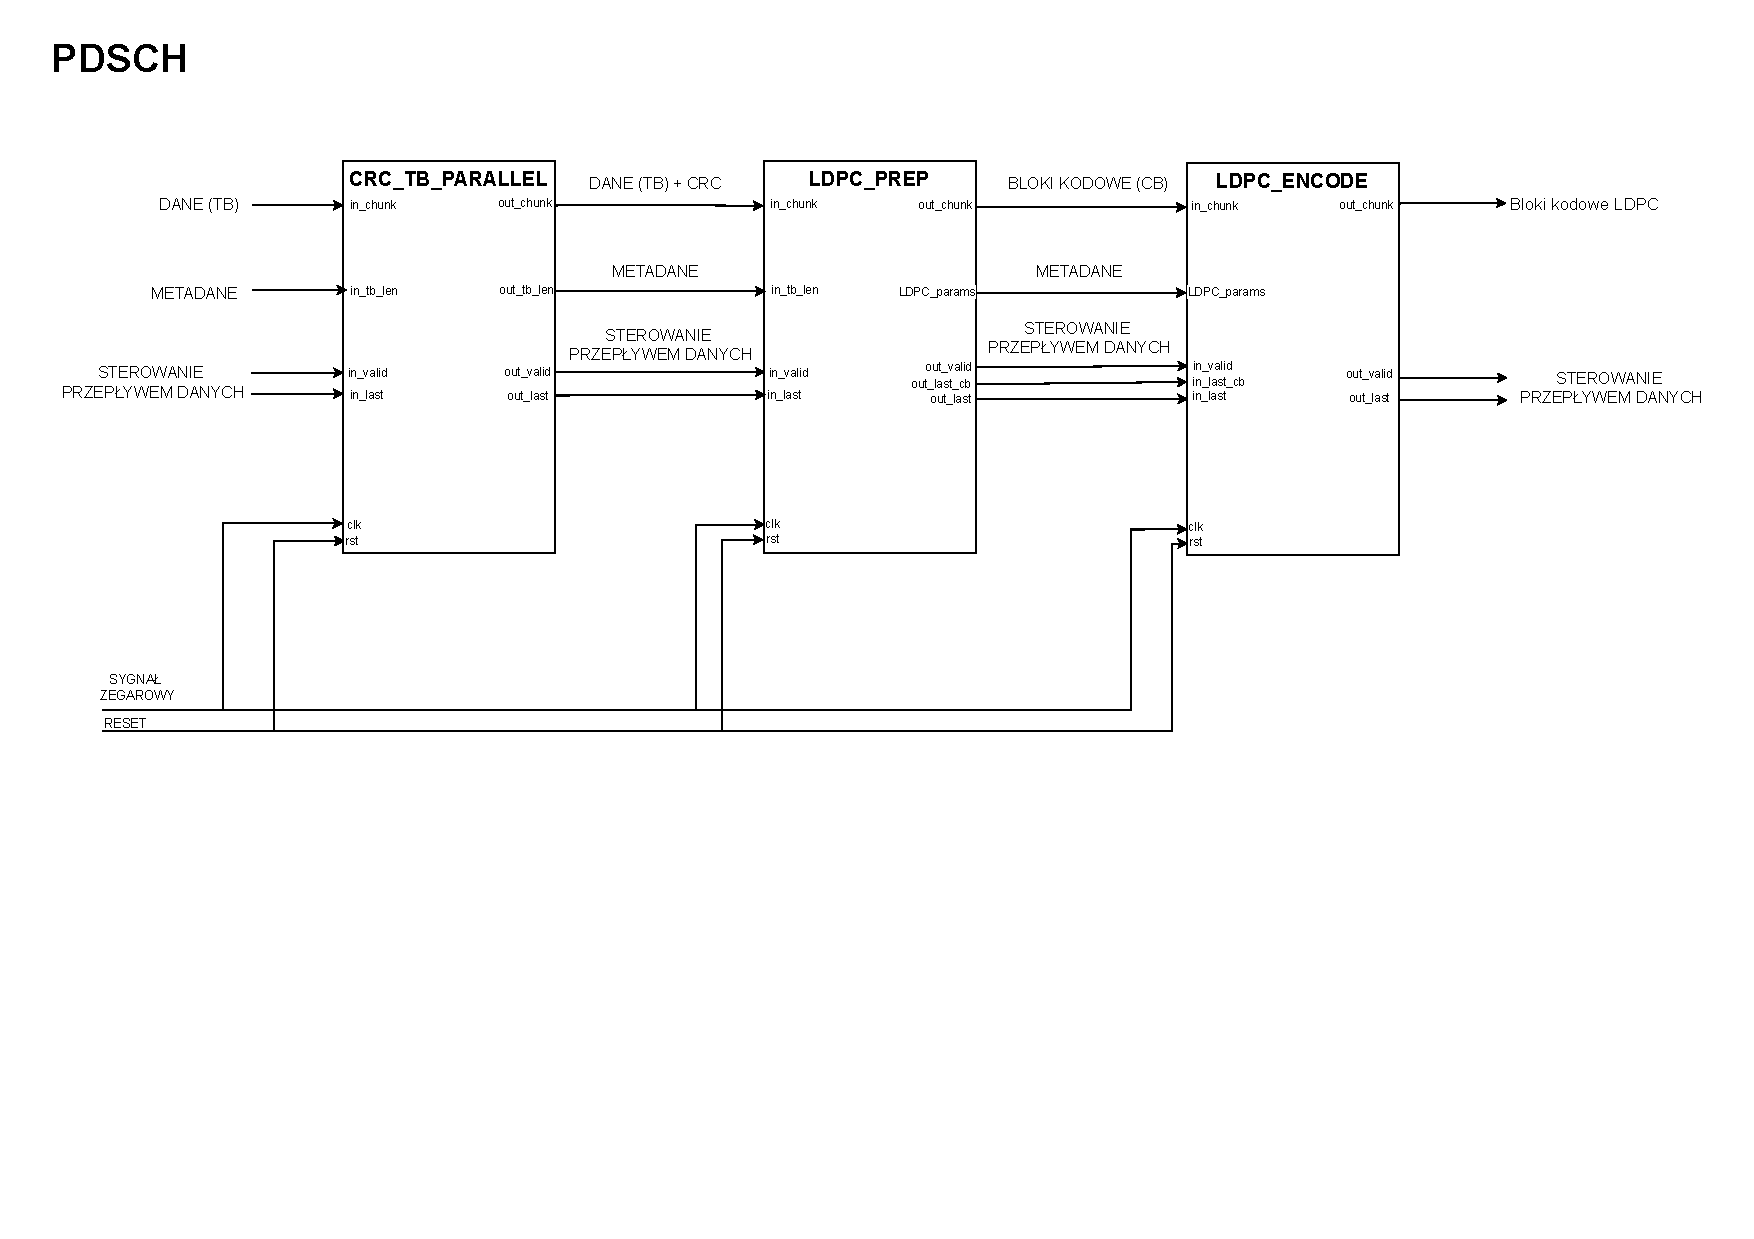
\includegraphics[width=0.98\linewidth]{./schematy/PDSCH.pdf}
\caption{Integracja toru w~module \texttt{PDSCHTx}.}
\label{fig:pdschtx_overview}
\end{figure}

\paragraph{Łączenie bloków i~przepływ danych.}
Wejściowy strumień TB (\texttt{in\_chunk}, \texttt{in\_valid}, \texttt{in\_last}, \texttt{in\_tb\_len}) jest w~pierwszym kroku kierowany do modułu \texttt{CRC\_TB\_PARALLEL}, który dopisuje CRC TB i~przekazuje dane dalej w~tym samym formacie strumieniowym. Następnie \texttt{LDPC\_PREP} wykonuje operacje przygotowawcze do kodowania LDPC (m.in. segmentację TB na CB oraz dopisanie CRC CB) i~generuje metadane sterujące kodowaniem (\texttt{LDPC\_params}).

Moduł \texttt{LDPC\_ENCODE} przyjmuje strumień bloków kodowych oraz odpowiadające im metadane i~realizuje kodowanie. Na wyjściu kodera powstaje pojedynczy strumień danych odpowiadający całemu TB po kodowaniu LDPC (z zachowaniem przyjętego w~projekcie sposobu emisji danych).

\paragraph{Sterowanie granicami TB i~CB.}
W top-level zastosowano rozdzielenie sygnałów końca ramki na dwa poziomy:
\begin{itemize}
  \item \textbf{Koniec TB} (\texttt{in\_last} / \texttt{out\_last}) -- występuje tylko raz dla całego bloku transportowego i~zamyka przetwarzanie całej ramki w~torze.
  \item \textbf{Koniec CB} (\texttt{out\_last\_cb}) -- sygnał wewnętrzny pomiędzy \texttt{LDPC\_PREP} i~\texttt{LDPC\_ENCODE}, służący do jednoznacznego oznaczania granicy kolejnych bloków kodowych w~strumieniu. Pozwala to koderowi poprawnie rozdzielać CB bez potrzeby dodatkowego „ręcznego” liczenia słów na wejściu.
\end{itemize}

Takie podejście upraszcza integrację: tor może traktować TB jako jedną ramkę wejściową, natomiast koder LDPC dostaje dodatkową informację o~końcu aktualnego CB, co jest naturalne w~kontekście segmentacji i~późniejszej rekombinacji danych.

Na poziomie \texttt{PDSCHTx} integracja sprowadza się więc do poprawnego połączenia sygnałów \texttt{valid/last} pomiędzy blokami oraz zapewnienia, że granice TB/CB są zachowane i~jednoznaczne na kolejnych etapach przetwarzania.

\paragraph{Reset i~cykl pracy toru.}
Reset (\texttt{rst}) jest wspólny dla całego toru i~inicjalizuje wszystkie etapy przetwarzania do stanu spoczynkowego. Zgodnie z~przyjętymi założeniami projektowymi tor obsługuje pojedynczy TB w~jednym cyklu pracy, a~rozpoczęcie przetwarzania następnego TB wymaga ponownego resetu.





















%%%%%%%%%%%%%%%%%%%%%
%% RYSUNEK Z PLIKU
%
%\begin{figure}
%\centering
%
\includegraphics[width=0.5\textwidth]{./graf/politechnika_sl_logo_bw_pion_pl.pdf}
%\caption{Podpis rysunku zawsze pod rysunkiem.}
%\label{fig:etykieta-rysunku}
%\end{figure}
%Rys. \ref{fig:etykieta-rysunku} przestawia …
%%%%%%%%%%%%%%%%%%%%%
%
%%%%%%%%%%%%%%%%%%%%%
%% WIELE RYSUNKÓW 
%
%\begin{figure}
%\centering
%\begin{subfigure}{0.4\textwidth}
%    
\includegraphics[width=\textwidth]{./graf/politechnika_sl_logo_bw_pion_pl.pdf}
%    \caption{Lewy górny rysunek.}
%    \label{fig:lewy-gorny}
%\end{subfigure}
%\hfill
%\begin{subfigure}{0.4\textwidth}
%    
\includegraphics[width=\textwidth]{./graf/politechnika_sl_logo_bw_pion_pl.pdf}
%    \caption{Prawy górny rysunek.}
%    \label{fig:prawy-gorny}
%\end{subfigure}
%
%\begin{subfigure}{0.4\textwidth}
%    
\includegraphics[width=\textwidth]{./graf/politechnika_sl_logo_bw_pion_pl.pdf}
%    \caption{Lewy dolny rysunek.}
%    \label{fig:lewy-dolny}
%\end{subfigure}
%\hfill
%\begin{subfigure}{0.4\textwidth}
%    
\includegraphics[width=\textwidth]{./graf/politechnika_sl_logo_bw_pion_pl.pdf}
%    \caption{Prawy dolny rysunek.}
%    \label{fig:prawy-dolny}
%\end{subfigure}
%        
%\caption{Wspólny podpis kilku rysunków.}
%\label{fig:wiele-rysunkow}
%\end{figure}
%Rys. \ref{fig:wiele-rysunkow} przestawia wiele ważnych informacji, np. rys. \ref{fig:prawy-gorny} jest na prawo u góry.
%%%%%%%%%%%%%%%%%%%%%


 
% \begin{figure}
% \centering
% \begin{tikzpicture}
% \begin{axis}[
%     y tick label style={
%         /pgf/number format/.cd,
%             fixed,   % po zakomentowaniu os rzednych jest indeksowana wykladniczo
%             fixed zerofill, % 1.0 zamiast 1
%             precision=1,
%         /tikz/.cd
%     },
%     x tick label style={
%         /pgf/number format/.cd,
%             fixed,
%             fixed zerofill,
%             precision=2,
%         /tikz/.cd
%     }
% ]
% \addplot [domain=0.0:0.1] {rnd};
% \end{axis} 
% \end{tikzpicture}
% \caption{Podpis rysunku po rysunkiem.}
% \label{fig:2}
% \end{figure}

